\documentclass[14pt]{extarticle}
\usepackage{natbib}

\usepackage{xcolor}
\usepackage{amsmath}
\newcommand{\tuple}[1]{ \langle #1 \rangle }
%\usepackage{automata}
\usepackage{times}
\usepackage{ltablex}
\usepackage{tasks}
\usepackage{threeparttable}
\usepackage{booktabs}
\usepackage{xcolor} % For custom colors
\usepackage{tcolorbox} % For colored box styling
\usepackage{amsmath, amsfonts, amssymb, amsthm} % Math related
\usepackage{natbib}
\usepackage{fontspec}
\usepackage{luatexja}
\usepackage[mathscr]{euscript}

%%%%%% Template
\usepackage{hyperref}
\hypersetup{colorlinks=true,allcolors=blue}

\usepackage{vmargin}
\setpapersize{USletter}
\setmarginsrb{1.0in}{1.0in}{1.0in}{0.6in}{0pt}{0pt}{0pt}{0.4in}

% HOW TO USE THE ABOVE:
%\setmarginsrb{leftmargin}{topmargin}{rightmargin}{bottommargin}{headheight}{headsep}{footheight}{footskip}
%\raggedbottom
% paragraphs indent & skip:
\parindent  0.3cm
\parskip    -0.01cm

\usepackage{tikz}
\usetikzlibrary{backgrounds}
\usetikzlibrary{decorations.pathreplacing, intersections, positioning}

% hyphenation:
% \hyphenpenalty=10000 % no hyphen
% \exhyphenpenalty=10000 % no hyphen
\sloppy

% notes-style paragraph spacing and indentation:
\usepackage{parskip}
\setlength{\parindent}{0cm}

% let derivations break across pages
\allowdisplaybreaks

\newcommand{\orange}[1]{\textcolor{orange}{#1}}
\newcommand{\blue}[1]{\textcolor{blue}{#1}}
\newcommand{\red}[1]{\textcolor{red}{#1}}
\newcommand{\freq}[1]{{\bf \sf F}(#1)}
\newcommand{\datafreq}[2]{{{\bf \sf F}_{#1}(#2)}}

\def\qqquad{\quad\qquad}
\def\qqqquad{\qquad\qquad}

%%%%%%%%%%%%%%%%%%%%%%%%%%%%%%%%%%%%%%%%%%%%%%%%%%%%%%%%%%%%%%%%%%%%%%%%%%%%%%%%
%%%%%%%%%%%%%%%%%%%%%%%%%%%%%%%%%%%%%%%%%%%%%%%%%%%%%%%%%%%%%%%%%%%%%%%%%%%%%%%%

% fill-in-blank question style, found in https://tex.stackexchange.com/a/505089

\usepackage{ifthen}
\usepackage{tocloft}
\usepackage{exercise}
% \usepackage{xcolor}

% Set the Show Answers Boolean
\newboolean{showAns}
\setboolean{showAns}{false}
\newcommand{\showAns}{\setboolean{showAns}{true}}

% The length of the Answer line
\newlength{\answerlength}
\newcommand{\anslen}[1]{\settowidth{\answerlength}{#1}}

% ans command that indicates space for an answer or shows the answer in red
\newcommand{\ans}[1]{\settowidth{\answerlength}{\hspace{2ex}#1\hspace{2ex}}%
    \ifthenelse{\boolean{showAns}}%
        {\textcolor{red}{\underline{\hspace{2ex}#1\hspace{2ex}}}}%
        {\underline{\hspace{\answerlength}}}}%

\newcommand{\details}[1]{\settowidth{\answerlength}{#1}%
    \ifthenelse{\boolean{showAns}}%
        {\begin{tcolorbox}[colback=blue!5!white,colframe=blue!75!black,title=Solution] #1 \end{tcolorbox}}%
        {}}%

% Formatting how multiple choices Questions are formated.
\settasks{label=(\Alph*), label-width=30pt}


% Some commands for the Exercise Question package
\renewcommand{\QuestionNB}{\Large\protect\textcircled{\small\bfseries\arabic{Question}}\ }
\renewcommand{\ExerciseHeader}{} %no header
\renewcommand{\QuestionBefore}{3ex} %Space above each Q
\setlength{\QuestionIndent}{8pt} % Indent after Q number


% To create the list of answers with tocloft...
\newcommand{\listanswername}{Answers}
\newlistof[Question]{answer}{Answers}{\listanswername}

% Creates a TOC for Answers
\newcounter{prevQ}
\newcommand{\answer}[1]{\refstepcounter{answer}%
\ans{#1}%
\ifnum\theQuestion=\theprevQ%
        \addcontentsline{Answers}{answer}{\protect\numberline{}#1}% don't include the Q number
        \else%
        \addcontentsline{Answers}{answer}{\protect\numberline{\theQuestion}#1}%
        \setcounter{prevQ}{\value{Question}}%
        \fi%
        }%

% \hyphenpenalty=10000 % no hyphen
% \exhyphenpenalty=10000 % no hyphen
\sloppy              % hyphen

\newcommand{\HRule}{\rule{\linewidth}{0.5mm}}
\newcommand{\Hrule}{\rule{\linewidth}{0.3mm}}

%tocloft formatting listofanswers
\renewcommand{\cftAnswerstitlefont}{\bfseries\large}
\renewcommand{\cftanswerdotsep}{\cftnodots}
\cftpagenumbersoff{answer}
\addtolength{\cftanswernumwidth}{10pt}

\makeatletter% since there's an at-sign (@) in the command name
\renewcommand{\@maketitle}{%
  \parindent=0pt% don't indent paragraphs in the title block
  \centering
  {\Large \bfseries\textsc{\@title}} \\
  \vspace{5pt}
  {\large \textit{\@author}} \\
  \HRule \\
  \vspace{1em}
}
\makeatother% resets the meaning of the at-sign (@)

\setmainfont{Crimson Pro Light}[
  ItalicFont={* Italic},
  BoldFont={Crimson Pro Medium},
  BoldItalicFont={Crimson Pro Medium Italic}]
\setsansfont{Crimson Pro Light}[
  ItalicFont={* Italic},
  BoldFont={Crimson Pro Medium},
  BoldItalicFont={Crimson Pro Medium Italic}]

\title{Final Exam}
\author{Macroeconomics I \\ Hui-Jun Chen}

\begin{document}

\maketitle

% \showAns
% \listofanswer


% % Due at 11:59 PM (Eastern Time) on Sunday, June 14, 2022.

% Please answer this problem set on Carmen quizzes ``Problem Set 2''. In the following problems, the part that is in \textbf{\red{red and bold}} are the order of questions that should be answered on Carmen quizzes.

\begin{Exercise}

\section*{Instruction}

\textbf{Each question worth 2.5 points. The total is 100.}


\section*{Question 1}
\label{sec:Question_1}
\addcontentsline{toc}{section}{Question 1}

Consider the two-period dynamic general equilibrium model with a representative consumer, representative firm and government.
The consumer values consumption and leisure in each period, $C$ and $l$, and provides labour, $N_{S}$, in return for a real wage, $w$. The consumer pays lump-sum taxes $ T $ each period and receives all profits from the firm, $\pi$.%

The representative firm uses labour and capital, $N_{D}$ and $K$, to produce output.
In the first period, it also chooses investment, $I$.
This determines its capital stock for production in the second period, $K^{\prime}$, through the capital accumulation equation $K^{\prime}=\left(  1-\delta\right)  K+I$.%

The consumer's preferences are
%
\begin{equation*}
    U(C, C', N, N') = u(C) - v(N_{S}) + u(C') - v(N'_{S})
,\end{equation*}
%
and the firm's technology is
%
\begin{equation*}
    Y = z F(K, N) = z K^{\alpha} N^{1-\alpha}, \text{ where } \alpha \in (0, 1)
.\end{equation*}
%
Lastly, recall that the government must balance its budget across the two periods, $G+\frac{G^{\prime}}{1+r}=T+\frac{T^{\prime} }{1+r}$, where $G$ is government spending and $T$ are taxes.



\Question \label{MRS} Assume assumption N1 holds, i.e., substitution effect dominates income effect from a change in real wage, then given interest rate $ r $, consumer will choose the quantity of labor supply $ N_{S} $ by \answer{A}
\begin{tasks}(2)
    \task $ MRS_{l, C} = w $
    \task $ MRS_{C, C'} = r $
    \task $ MRS_{l, C} = r $
    \task $ MRS_{C, C'} = w $
\end{tasks}

\Question where the $ MRS $ in question \ref{MRS} is \answer{C}
\begin{tasks}(2)
    \task $ MRS_{l, C} = \frac{u'(C)}{u'(C')} $
    \task $ MRS_{C, C'} = \frac{u'(C)}{u'(C')}$
    \task $ MRS_{l, C} = \frac{v'(N_{S})}{u'(C)} $
    \task $ MRS_{C, C'} = \frac{v'(N_{S})}{u'(C)} $
\end{tasks}

\Question Following assumption N1, the slope of the labor supply is \answer{D} in wage and thus the labor supply curve has \answer{D} slope
\begin{tasks}(2)
    \task decreasing; positive
    \task increasing; negative
    \task decreasing; negative
    \task increasing; positive
\end{tasks}

\Question Following assumption N2, how does the labor supply curve response to a rise in real interest rate $ r $? \answer{B}
\begin{tasks}(2)
    \task shift to the left
    \task shift to the right
    \task not affected
    \task ambiguous
\end{tasks}

\Question In the firm's labor demand, what is the equation that can determine the labor demand curve? \answer{A}
\begin{tasks}(2)
    \task $ MPN = w $
    \task $ MPK = r $
    \task $ MPN = r $
    \task $ MPK = w $
\end{tasks}


\Question How does a fall in total factor productivity $ z $ affect the equilibrium in labor market? \answer{B}
\begin{tasks}(1)
    \task labor supply will shift to the left; labor demand will shift to the right
    \task labor supply will shift to the right; labor demand will shift to the left
    \task labor supply will shift to the right; labor demand not shift
    \task labor supply will not shift; labor demand will shift to the left
\end{tasks}

\Question For the goods demand, what is the optimal investment schedule? \answer{D}
\begin{tasks}(2)
    \task $ MPN' - \delta = w $
    \task $ MPN' - \delta = r $
    \task $ MPK' - w = r $
    \task $ MPK' - \delta = r $
\end{tasks}

\Question how does a rise in the real interest rate $ r $ changes the investment? \answer{C}
\begin{tasks}(2)
    \task $ I^{d} \uparrow  $
    \task $ I^{d} $ unchanged
    \task $ I^{d} \downarrow  $
    \task $ I^{d} $ movement is ambiguous
\end{tasks}

% A: z', B: z, C: K, D: G
\Question \label{z'} Consider a rise in future total factor productivity $ z' $. Which of the following figure correctly represents the movement of labor and goods market? \answer{A}
\begin{tasks}(1)
    \task

        \begin{minipage}{0.5\textwidth}
            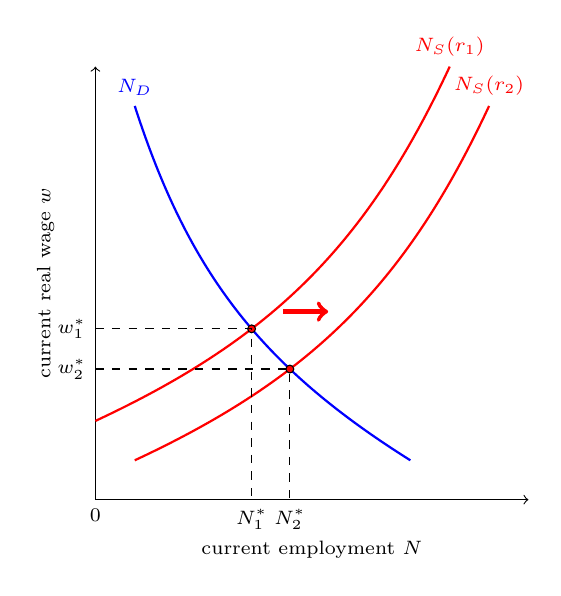
\begin{tikzpicture}[domain=0:5]
                \tikzstyle{every node}=[font=\scriptsize]
                \pgfmathsetmacro{\x}{5};
                \pgfmathsetmacro{\y}{5};
                % \draw[very thin,color=gray, step=0.1] (0,0) grid (\x, \y); % gray grid
                \draw[->] (0,0) node[below]{ $ 0 $  } -- node[below, yshift = -0.4cm]{current employment $ N $} (\x + 0.5,0) ;   % label x axis
                \draw[->] (0,0) -- node[above, rotate=90, yshift = 0.4cm]{current real wage $w$} (0,\y + 0.5) ;   % label y axis
                \draw[thick, red, xshift = -0.5cm, yshift = 0.5cm, name path = aaa]
                    (\x, \y)
                    node[above]{$N_{S}( r_{1} )$}
                    to[bend left=20]
                    node[pos=0.6] (AA) {}
                    (0.5, 0.5);
                \draw[thick, red, name path = aa]
                    (\x, \y)
                    node[above]{$N_{S}( r_{2} )$}
                    to[bend left=20]
                    (0.5, 0.5);
                \draw[thick, blue, name path = bb]
                    (0.5, \y)
                    node[above]{$N_{D}$}
                    to[bend right=20]
                    (4, 0.5);
                \path[name intersections={of=aa and bb, by=b}];
                \path[name intersections={of=aaa and bb, by=bb}];
                \node[draw,fill=red,circle,inner sep=1pt] at (b) {};
                \node[draw,fill=red,circle,inner sep=1pt] at (bb) {};
                \draw[->, ultra thick, red] (AA) -- ++(0.7, 0);
                \path (bb); \pgfgetlastxy{\xcoord}{\ycoord};
                \coordinate (bb_x) at (\xcoord, 0);
                \coordinate (bb_y) at (0, \ycoord);
                \draw[dashed] (bb_y) node[left]{$w_{1}^{*}$}  -- (bb) -- (bb_x) node[below]{$N_{1}^{*}$};
                \path (b); \pgfgetlastxy{\xcoord}{\ycoord};
                \coordinate (b_x) at (\xcoord, 0);
                \coordinate (b_y) at (0, \ycoord);
                \draw[dashed] (b_y) node[left]{$w_{2}^{*}$}  -- (b) -- (b_x) node[below]{$N_{2}^{*}$};

            \end{tikzpicture}
        \end{minipage}
        \begin{minipage}{0.5\textwidth}

            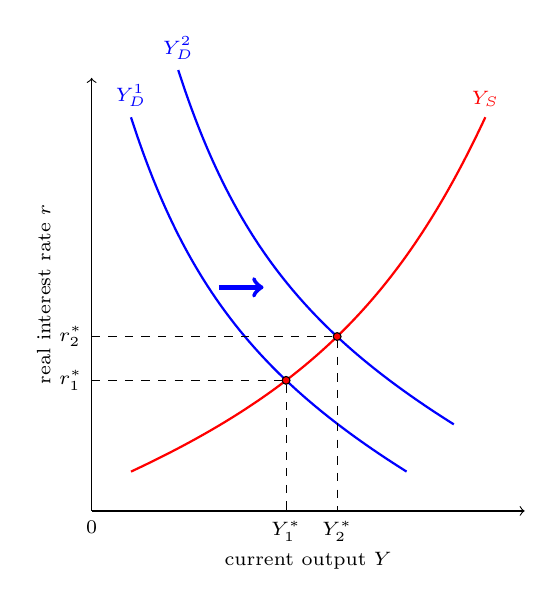
\begin{tikzpicture}[domain=0:5]
                \tikzstyle{every node}=[font=\scriptsize]
                \pgfmathsetmacro{\x}{5};
                \pgfmathsetmacro{\y}{5};
                % \draw[very thin,color=gray, step=0.1] (0,0) grid (\x, \y); % gray grid
                \draw[->] (0,0) node[below]{ $ 0 $  } -- node[below, yshift = -0.4cm]{current output $ Y $} (\x + 0.5,0) ;   % label x axis
                \draw[->] (0,0) -- node[above, rotate=90, yshift = 0.4cm]{real interest rate $r$} (0,\y + 0.5) ;   % label y axis
                \draw[thick, red, name path = aa]
                    (\x, \y)
                    node[above]{$Y_{S}$}
                    to[bend left=20]
                    (0.5, 0.5);
                \draw[thick, blue, name path = bb]
                    (0.5, \y)
                    node[above]{$Y_{D}^{1}$}
                    to[bend right=20]
                    node[pos = 0.4] (BB) {}
                    (4, 0.5);
                \draw[thick, blue, xshift = 0.6cm, yshift = 0.6cm, name path = bbb]
                    (0.5, \y)
                    node[above]{$Y_{D}^{2}$}
                    to[bend right=20]
                    (4, 0.5);
                \path[name intersections={of=aa and bb, by=a}];
                \path[name intersections={of=aa and bbb, by=bbb}];
                \node[draw,fill=red,circle,inner sep=1pt] at (a) {};
                \node[draw,fill=red,circle,inner sep=1pt] at (bbb) {};
                \draw[->, ultra thick, blue] (BB) -- ++(0.7, 0);
                \path (a); \pgfgetlastxy{\xcoord}{\ycoord};
                \coordinate (a_x) at (\xcoord, 0);
                \coordinate (a_y) at (0, \ycoord);
                \draw[dashed] (a_y) node[left]{$r_{1}^{*}$}  -- (a) -- (a_x) node[below]{$Y_{1}^{*}$};
                \path (bbb); \pgfgetlastxy{\xcoord}{\ycoord};
                \coordinate (bbb_x) at (\xcoord, 0);
                \coordinate (bbb_y) at (0, \ycoord);
                \draw[dashed] (bbb_y) node[left]{$r_{2}^{*}$}  -- (bbb) -- (bbb_x) node[below]{$Y_{2}^{*}$};

            \end{tikzpicture}
        \end{minipage}

    \task

        \begin{minipage}{0.5\textwidth}
            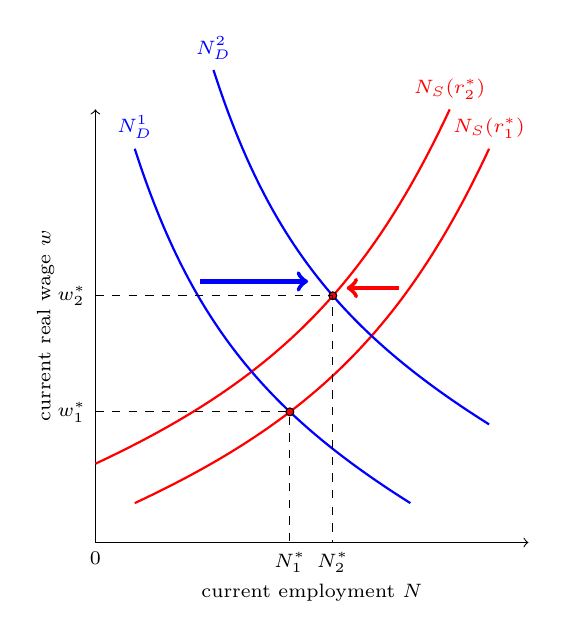
\begin{tikzpicture}[domain=0:5]
                \tikzstyle{every node}=[font=\scriptsize]
                \pgfmathsetmacro{\x}{5};
                \pgfmathsetmacro{\y}{5};
                % \draw[very thin,color=gray, step=0.1] (0,0) grid (\x, \y); % gray grid
                \draw[->] (0,0) node[below]{ $ 0 $  } -- node[below, yshift = -0.4cm]{current employment $ N $} (\x + 0.5,0) ;   % label x axis
                \draw[->] (0,0) -- node[above, rotate=90, yshift = 0.4cm]{current real wage $w$} (0,\y + 0.5) ;   % label y axis
                \draw[thick, red, name path = aa]
                    (\x, \y)
                    node[above]{$N_{S}( r_{1}^{*} )$}
                    to[bend left=20]
                    node[pos=0.3] (AA) {}
                    (0.5, 0.5);
                \draw[thick, red, xshift = -0.5cm, yshift = 0.5cm, name path = dd]
                    (\x, \y)
                    node[above]{$N_{S}( r_{2}^{*} )$}
                    to[bend left=20]
                    (0.5, 0.5);
                \draw[thick, blue, name path = bb]
                    (0.5, \y)
                    node[above]{$N_{D}^{1}$}
                    to[bend right=20]
                    node[pos=0.3] (BB) {}
                    (4, 0.5);
                \draw[thick, blue, xshift = 1cm, yshift = 1cm, name path = cc]
                    (0.5, \y)
                    node[above]{$N_{D}^{2}$}
                    to[bend right=20]
                    (4, 0.5);
                \path[name intersections={of=aa and bb, by=b}];
                \path[name intersections={of=dd and cc, by=c}];
                \node[draw,fill=red,circle,inner sep=1pt] at (b) {};
                \node[draw,fill=red,circle,inner sep=1pt] at (c) {};
                \draw[->, ultra thick, blue] (BB) -- ++(1.5, 0);
                \draw[->, ultra thick, red] (AA) -- ++(-0.8, 0);
                \path (b); \pgfgetlastxy{\xcoord}{\ycoord};
                \coordinate (b_x) at (\xcoord, 0);
                \coordinate (b_y) at (0, \ycoord);
                \path (c); \pgfgetlastxy{\xcoord}{\ycoord};
                \coordinate (c_x) at (\xcoord, 0);
                \coordinate (c_y) at (0, \ycoord);
                \draw[dashed] (b_y) node[left]{$w_{1}^{*}$}  -- (b) -- (b_x) node[below]{$N_{1}^{*}$};
                \draw[dashed] (c_y) node[left]{$w_{2}^{*}$}  -- (c) -- (c_x) node[below]{$N_{2}^{*}$};

            \end{tikzpicture}
        \end{minipage}
        \begin{minipage}{0.5\textwidth}

            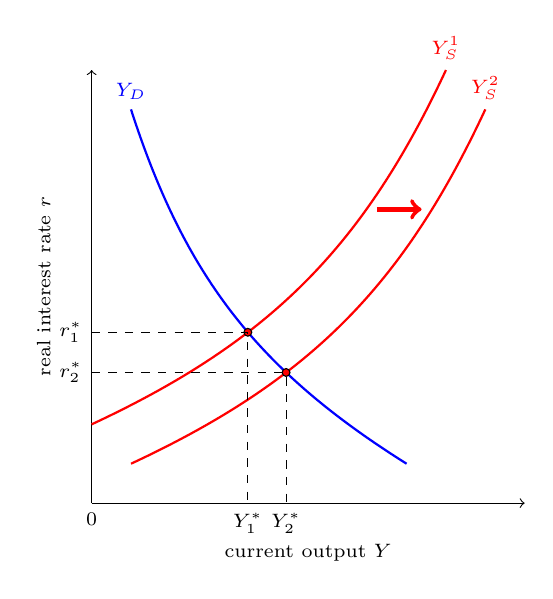
\begin{tikzpicture}[domain=0:5]
                \tikzstyle{every node}=[font=\scriptsize]
                \pgfmathsetmacro{\x}{5};
                \pgfmathsetmacro{\y}{5};
                % \draw[very thin,color=gray, step=0.1] (0,0) grid (\x, \y); % gray grid
                \draw[->] (0,0) node[below] {$ 0 $} -- node[below, yshift = -0.4cm]{current output $ Y $} (\x + 0.5,0) ;   % label x axis
                \draw[->] (0,0) -- node[above, rotate=90, yshift = 0.4cm]{real interest rate $r$} (0,\y + 0.5) ;   % label y axis
                \draw[thick, red, name path = aa]
                    (\x, \y)
                    node[above]{$Y_{S}^{2}$}
                    to[bend left=20]
                    (0.5, 0.5);
                \draw[thick, red, xshift = -0.5cm, yshift = 0.5cm, name path = cc]
                    (\x, \y)
                    node[above]{$Y_{S}^{1}$}
                    to[bend left=20]
                    node[pos=0.3] (AA) {}
                    (0.5, 0.5);
                \draw[thick, blue, name path = bb]
                    (0.5, \y)
                    node[above]{$Y_{D}$}
                    to[bend right=20]
                    (4, 0.5);
                \path[name intersections={of=aa and bb, by=a}];
                \path[name intersections={of=bb and cc, by=c}];
                \node[draw,fill=red,circle,inner sep=1pt] at (a) {};
                \node[draw,fill=red,circle,inner sep=1pt] at (c) {};
                \draw[->, ultra thick, red] (AA) -- ++(0.7, 0);
                \path (a); \pgfgetlastxy{\xcoord}{\ycoord};
                \coordinate (a_x) at (\xcoord, 0);
                \coordinate (a_y) at (0, \ycoord);
                \path (c); \pgfgetlastxy{\xcoord}{\ycoord};
                \coordinate (c_x) at (\xcoord, 0);
                \coordinate (c_y) at (0, \ycoord);
                \draw[dashed] (a_y) node[left]{$r_{2}^{*}$}  -- (a) -- (a_x) node[below]{$Y_{2}^{*}$};
                \draw[dashed] (c_y) node[left]{$r_{1}^{*}$}  -- (c) -- (c_x) node[below]{$Y_{1}^{*}$};
            \end{tikzpicture}
        \end{minipage}

    \task

        \begin{minipage}{0.5\textwidth}
            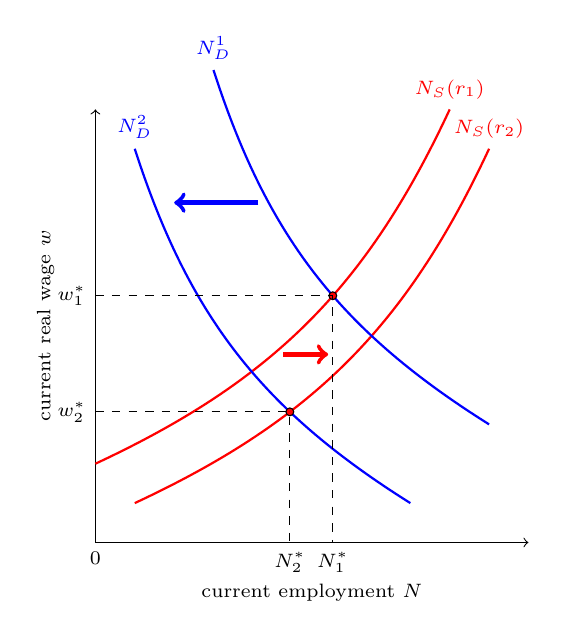
\begin{tikzpicture}[domain=0:5]
                \tikzstyle{every node}=[font=\scriptsize]
                \pgfmathsetmacro{\x}{5};
                \pgfmathsetmacro{\y}{5};
                % \draw[very thin,color=gray, step=0.1] (0,0) grid (\x, \y); % gray grid
                \draw[->] (0,0) node[below]{ $ 0 $  } -- node[below, yshift = -0.4cm]{current employment $ N $} (\x + 0.5,0) ;   % label x axis
                \draw[->] (0,0) -- node[above, rotate=90, yshift = 0.4cm]{current real wage $w$} (0,\y + 0.5) ;   % label y axis
                \draw[thick, red, xshift = -0.5cm, yshift = 0.5cm, name path = aaa]
                    (\x, \y)
                    node[above]{$N_{S}( r_{1} )$}
                    to[bend left=20]
                    node[pos=0.6] (AA) {}
                    (0.5, 0.5);
                \draw[thick, red, name path = aa]
                    (\x, \y)
                    node[above]{$N_{S}( r_{2} )$}
                    to[bend left=20]
                    (0.5, 0.5);
                \draw[thick, blue, xshift = 1cm, yshift = 1cm, name path = bbb]
                    (0.5, \y)
                    node[above]{$N_{D}^{1}$}
                    to[bend right=20]
                    node[pos = 0.3] (BB) {}
                    (4, 0.5);
                \draw[thick, blue, name path = bb]
                    (0.5, \y)
                    node[above]{$N_{D}^{2}$}
                    to[bend right=20]
                    (4, 0.5);
                \path[name intersections={of=aa and bb, by=b}];
                \path[name intersections={of=aaa and bbb, by=bb}];
                \node[draw,fill=red,circle,inner sep=1pt] at (b) {};
                \node[draw,fill=red,circle,inner sep=1pt] at (bb) {};
                \draw[->, ultra thick, red] (AA) -- ++(0.7, 0);
                \draw[->, ultra thick, blue] (BB) -- ++(-1.2, 0);
                \path (bb); \pgfgetlastxy{\xcoord}{\ycoord};
                \coordinate (bb_x) at (\xcoord, 0);
                \coordinate (bb_y) at (0, \ycoord);
                \draw[dashed] (bb_y) node[left]{$w_{1}^{*}$}  -- (bb) -- (bb_x) node[below]{$N_{1}^{*}$};
                \path (b); \pgfgetlastxy{\xcoord}{\ycoord};
                \coordinate (b_x) at (\xcoord, 0);
                \coordinate (b_y) at (0, \ycoord);
                \draw[dashed] (b_y) node[left]{$w_{2}^{*}$}  -- (b) -- (b_x) node[below]{$N_{2}^{*}$};

            \end{tikzpicture}
        \end{minipage}
        \begin{minipage}{0.5\textwidth}

            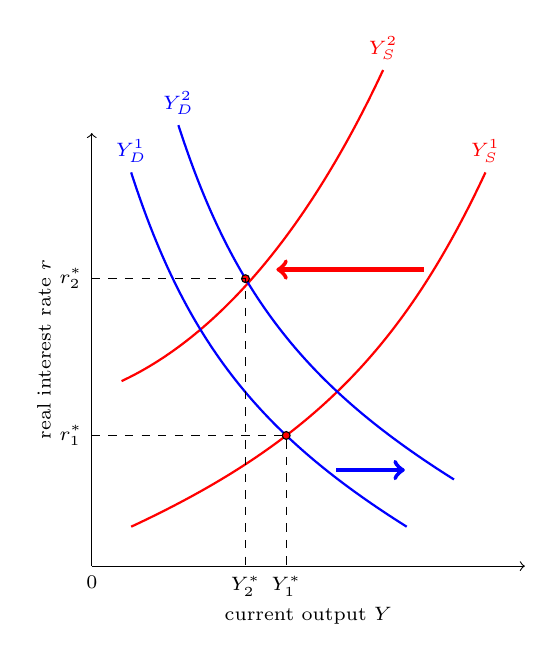
\begin{tikzpicture}[domain=0:5]
                \tikzstyle{every node}=[font=\scriptsize]
                \pgfmathsetmacro{\x}{5};
                \pgfmathsetmacro{\y}{5};
                % \draw[very thin,color=gray, step=0.1] (0,0) grid (\x, \y); % gray grid
                \draw[->] (0,0) node[below]{ $ 0 $  } -- node[below, yshift = -0.4cm]{current output $ Y $} (\x + 0.5,0) ;   % label x axis
                \draw[->] (0,0) -- node[above, rotate=90, yshift = 0.4cm]{real interest rate $r$} (0,\y + 0.5) ;   % label y axis
                \draw[thick, red, name path = aa]
                    (\x, \y)
                    node[above]{$Y_{S}^{1}$}
                    to[bend left=20]
                    node[pos = 0.2] (AA) {}
                    (0.5, 0.5);
                \draw[thick, red, xshift = -1.3cm, yshift = 1.3cm, name path = aaa, shorten >= 1.3cm]
                    (\x, \y)
                    node[above]{$Y_{S}^{2}$}
                    to[bend left=20]
                    (0.5, 0.5);
                \draw[thick, blue, name path = bb]
                    (0.5, \y)
                    node[above]{$Y_{D}^{1}$}
                    to[bend right=20]
                    node[pos = 0.8] (BB) {}
                    (4, 0.5);
                \draw[thick, blue, xshift = 0.6cm, yshift = 0.6cm, name path = bbb]
                    (0.5, \y)
                    node[above]{$Y_{D}^{2}$}
                    to[bend right=20]
                    (4, 0.5);
                \path[name intersections={of=aa and bb, by=a}];
                \path[name intersections={of=aaa and bbb, by=bbb}];
                \node[draw,fill=red,circle,inner sep=1pt] at (a) {};
                \node[draw,fill=red,circle,inner sep=1pt] at (bbb) {};
                \draw[->, ultra thick, blue] (BB) -- ++(1, 0);
                \draw[->, ultra thick, red] (AA) -- ++(-2, 0);
                \path (a); \pgfgetlastxy{\xcoord}{\ycoord};
                \coordinate (a_x) at (\xcoord, 0);
                \coordinate (a_y) at (0, \ycoord);
                \draw[dashed] (a_y) node[left]{$r_{1}^{*}$}  -- (a) -- (a_x) node[below]{$Y_{1}^{*}$};
                \path (bbb); \pgfgetlastxy{\xcoord}{\ycoord};
                \coordinate (bbb_x) at (\xcoord, 0);
                \coordinate (bbb_y) at (0, \ycoord);
                \draw[dashed] (bbb_y) node[left]{$r_{2}^{*}$}  -- (bbb) -- (bbb_x) node[below]{$Y_{2}^{*}$};

            \end{tikzpicture}
        \end{minipage}

    \task

        \begin{minipage}{0.5\textwidth}
            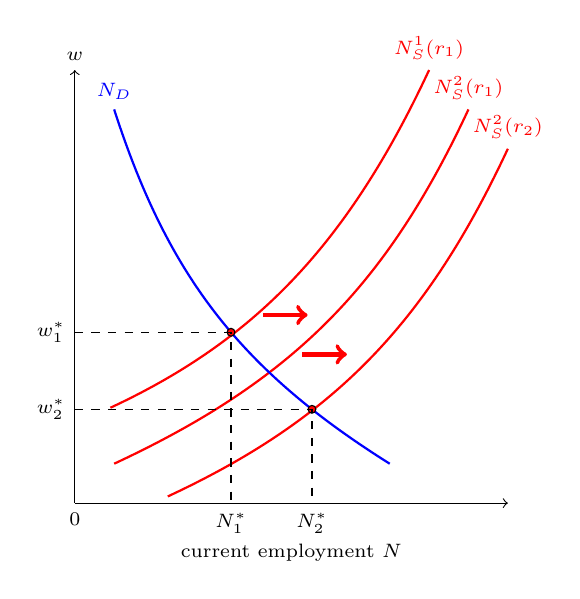
\begin{tikzpicture}[domain=0:5]
                \tikzstyle{every node}=[font=\scriptsize]
                \pgfmathsetmacro{\x}{5};
                \pgfmathsetmacro{\y}{5};
                % \draw[very thin,color=gray, step=0.1] (0,0) grid (\x, \y); % gray grid
                \draw[->] (0,0) node[below]{ $ 0 $  } -- node[below, yshift = -0.4cm]{current employment $ N $} (\x + 0.5,0) ;   % label x axis
                \draw[->] (0,0) -- (0,\y + 0.5) node[above]{$w$} ;   % label y axis
                \draw[thick, red, xshift = -0.5cm, yshift = 0.5cm, name path = aaa, shorten >= 0.5cm]
                    (\x, \y)
                    node[above]{$N_{S}^{1}( r_{1} )$}
                    to[bend left=20]
                    node[pos=0.6] (AA) {}
                    (0.5, 0.5);
                \draw[thick, red, name path = aa]
                    (\x, \y)
                    node[above]{$N_{S}^{2}( r_{1} )$}
                    to[bend left=20]
                    node[pos=0.6] (AAA) {}
                    (0.5, 0.5);
                \draw[thick, red, xshift = 0.5cm, yshift = -0.5cm, name path = aaaa, shorten >= 0.2cm]
                    (\x, \y)
                    node[above]{$N_{S}^{2}( r_{2} )$}
                    to[bend left=20]
                    (0.5, 0.5);
                \draw[thick, blue, name path = bb]
                    (0.5, \y)
                    node[above]{$N_{D}$}
                    to[bend right=20]
                    (4, 0.5);
                \path[name intersections={of=aaaa and bb, by=b}];
                \path[name intersections={of=aaa and bb, by=bb}];
                \node[draw,fill=red,circle,inner sep=1pt] at (b) {};
                \node[draw,fill=red,circle,inner sep=1pt] at (bb) {};
                \draw[->, ultra thick, red] (AA) -- ++(0.7, 0);
                \draw[->, ultra thick, red] (AAA) -- ++(0.7, 0);
                \path (bb); \pgfgetlastxy{\xcoord}{\ycoord};
                \coordinate (bb_x) at (\xcoord, 0);
                \coordinate (bb_y) at (0, \ycoord);
                \draw[dashed] (bb_y) node[left]{$w_{1}^{*}$}  -- (bb) -- (bb_x) node[below]{$N_{1}^{*}$};
                \path (b); \pgfgetlastxy{\xcoord}{\ycoord};
                \coordinate (b_x) at (\xcoord, 0);
                \coordinate (b_y) at (0, \ycoord);
                \draw[dashed] (b_y) node[left]{$w_{2}^{*}$}  -- (b) -- (b_x) node[below]{$N_{2}^{*}$};

            \end{tikzpicture}
        \end{minipage}
        \begin{minipage}{0.5\textwidth}

            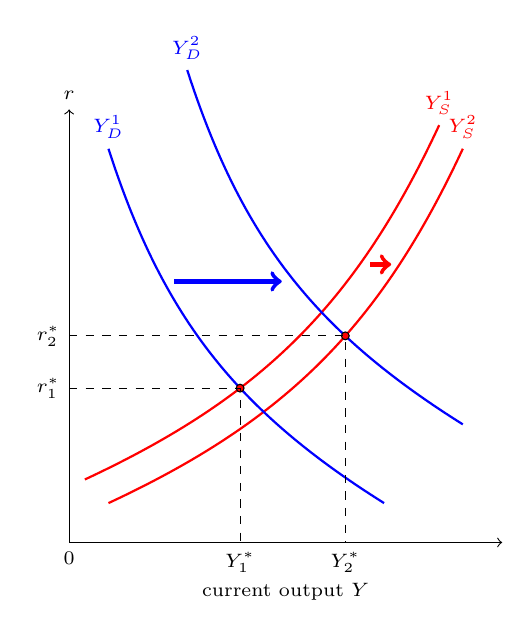
\begin{tikzpicture}[domain=0:5]
                \tikzstyle{every node}=[font=\scriptsize]
                \pgfmathsetmacro{\x}{5};
                \pgfmathsetmacro{\y}{5};
                % \draw[very thin,color=gray, step=0.1] (0,0) grid (\x, \y); % gray grid
                \draw[->] (0,0) node[below]{ $ 0 $  } -- node[below, yshift = -0.4cm]{current output $ Y $} (\x + 0.5,0) ;   % label x axis
                \draw[->] (0,0) -- (0,\y + 0.5) node[above]{$r$} ;   % label y axis
                \draw[thick, red, xshift = -0.3cm, yshift = 0.3cm, name path = aaa]
                    (\x, \y)
                    node[above]{$Y_{S}^{1}$}
                    to[bend left=20]
                    node[pos = 0.3] (AA) {}
                    (0.5, 0.5);
                \draw[thick, red, name path = aa]
                    (\x, \y)
                    node[above]{$Y_{S}^{2}$}
                    to[bend left=20]
                    (0.5, 0.5);
                \draw[thick, blue, name path = bb]
                    (0.5, \y)
                    node[above]{$Y_{D}^{1}$}
                    to[bend right=20]
                    node[pos = 0.3] (BB) {}
                    (4, 0.5);
                \draw[thick, blue, xshift = 1cm, yshift = 1cm, name path = bbb]
                    (0.5, \y)
                    node[above]{$Y_{D}^{2}$}
                    to[bend right=20]
                    (4, 0.5);
                \path[name intersections={of=aaa and bb, by=a}];
                \path[name intersections={of=aa and bbb, by=bbb}];
                \node[draw,fill=red,circle,inner sep=1pt] at (a) {};
                \node[draw,fill=red,circle,inner sep=1pt] at (bbb) {};
                \draw[->, ultra thick, blue] (BB) -- ++(1.5, 0);
                \draw[->, ultra thick, red] (AA) -- ++(0.4, 0);
                \path (a); \pgfgetlastxy{\xcoord}{\ycoord};
                \coordinate (a_x) at (\xcoord, 0);
                \coordinate (a_y) at (0, \ycoord);
                \draw[dashed] (a_y) node[left]{$r_{1}^{*}$}  -- (a) -- (a_x) node[below]{$Y_{1}^{*}$};
                \path (bbb); \pgfgetlastxy{\xcoord}{\ycoord};
                \coordinate (bbb_x) at (\xcoord, 0);
                \coordinate (bbb_y) at (0, \ycoord);
                \draw[dashed] (bbb_y) node[left]{$r_{2}^{*}$}  -- (bbb) -- (bbb_x) node[below]{$Y_{2}^{*}$};

            \end{tikzpicture}
        \end{minipage}
\end{tasks}

% A: z', B: z, C: K, D: G
\Question Using the same figures as in the choice of \ref{z'}, consider a rise in current total factor productivity $ z $. Which of the following figure correctly represents the movement of labor and goods market? \answer{B}

\Question Using the same figures as in the choice of \ref{z'}, consider a rise in government spending $ G $. Which of the following figure correctly represents the movement of labor and goods market? \answer{D}

\Question Using the same figures as in the choice of \ref{z'}, consider a decrease in capital endowment $ K $. Which of the following figure correctly represents the movement of labor and goods market? \answer{C}


\section*{Question 2}
\label{sec:Question_2}
\addcontentsline{toc}{section}{Question 2}

Consider a model that is \textbf{similar to} (not exactly!) the Lecture 14 Consumer Problem, but there are three differences:

\begin{enumerate}
    \item Consumers' utility function is given by $ U(C, C', N_{S}, N_{S}') = \log C - b N_{S} + \log C' - b N_{S}' $
    \item Consumers do \textbf{not} own the whole firm, i.e., $ \pi = 0 $. Instead, they buy shares of the firm \blue{$ s $} in date $ 0 $ to achieve intertemporal saving at per-unit price \blue{$ q $}. At date $ 1 $, consumers redeem their share to the firm and get \blue{$ s $} of reward.
    \item Consumers are \textbf{not} subject to the lump-sum tax, i.e., $ T = 0 $.
\end{enumerate}

\subsection*{Budget Constraint}
\label{sub:Budget_Constraint}
\addcontentsline{toc}{subsection}{Budget Constraint}

Firstly, let's follow the slide and think about the consumer's budget constraint, you can refer to Lecture 14, slide 4.

\Question there are $ \answer{A} $ choice variables,
    \begin{tasks}(4)
        \task $ 5 $
        \task $ 3 $
        \task $ 2 $
        \task $ 4 $
    \end{tasks}
\Question and they are $ \{C, C', N_{S}, N_{S}', \answer{C} \} $
    \begin{tasks}(4)
        \task $ S $
        \task $ S' $
        \task $ s $
        \task $ s' $
    \end{tasks}

\Question consumers own \textbf{part} of the firm and get $ \answer{B} $  of reward
    \begin{tasks}(4)
        \task $ \pi $
        \task $ s $
        \task $ \pi' $
        \task $ S $
    \end{tasks}

\Question and they are taken the equilibrium price $ \{w, w', \answer{D}\} $ as given.
    \begin{tasks}(4)
        \task $ r $
        \task $ r' $
        \task $ q' $
        \task $ q $
    \end{tasks}

After defining all of the variables, consumer's budget constraints in each period are

\Question date $ 0 $ budget constraints is \answer{$A$}
    \begin{tasks}(2)
        \task $ C + q s  = w N_{S}$
        \task $ C + S = w N_{S} + \pi - T $
        \task $ C = w N_{S} + qs $
        \task $ C = w N_{S} + \frac{s}{q} + \pi - T $
    \end{tasks}

\Question date $ 1 $ budget constraints is \answer{$C$}
    \begin{tasks}(2)
        \task $ C' = w N_{S} + \pi' - T' + (1+r)S$
        \task $ C' = w' N_{S}' + q s $
        \task $ C' = w' N_{S}' + s$
        \task $ C' = w' N_{S}' + \frac{s'}{q'} + \pi' - T' $
    \end{tasks}


\Question \label{LifeTimeBudget} The lifetime budget constraint by combining date $ 0 $ and date $ 1 $ budget constraints is \answer{$D$}
    \begin{tasks}(1)
        \task $ C + \frac{C'}{1+r} = w N_{S} + \frac{w' N_{S}'}{1+r} $
        \task $ C + \frac{C'}{1+r} = w N_{S} + \pi - T + \frac{w' N_{S}' + \pi' - T'}{1+r} $
        \task $ C - qC' = w N_{S} - q w' N_{S}' $
        \task $ C + qC' = w N_{S} + q w' N_{S}' $
    \end{tasks}

    Some calculation details:

    ~\answer{ $ s = C' - w' N_{S}' \Rightarrow C + q (C' - w' N_{S}') = w N_{S}$  }

    ~\answer{ $ \Rightarrow C + qC' = w N_{S} + q w' N_{S}' $ }

\subsection*{Preference}
\label{sub:Preference}
\addcontentsline{toc}{subsection}{Preference}

After finishing consumer's budget constraint, let's turn to the analysis preference:

\Question Accroding to the consumer's utility mentioned before, the derivative of consumer's utility function $ U(C, C', N_{S}, N_{S}') $ with respect to current consumption $ C $ is \answer{$A$}

    \begin{tasks}(4)
        \task $ \frac{1}{C} $
        \task $ \frac{1}{C'} $
        \task $ \frac{C'}{C} $
        \task $ \frac{C}{C'} $
    \end{tasks}

\Question Similarly, the derivative of consumer's utility function $ U(C, C', N_{S}, N_{S}') $ with respect to future consumption $ C' $ is \answer{$B$}

    \begin{tasks}(4)
        \task $ \frac{1}{C} $
        \task $ \frac{1}{C'} $
        \task $ \frac{C'}{C} $
        \task $ \frac{C}{C'} $
    \end{tasks}

\Question Similarly, the derivative of consumer's utility function $ U(C, C', N_{S}, N_{S}') $ with respect to current labor supply $ N_{S} $ is \answer{$D$}

    \begin{tasks}(4)
        \task $ \frac{1}{N_{S}'} $
        \task $ \frac{1}{N_{S}} $
        \task $ -b N_{S} $
        \task $ -b $
    \end{tasks}

\Question Similarly, the derivative of consumer's utility function $ U(C, C', N_{S}, N_{S}') $ with respect to future labor supply $ N_{S}' $ is \answer{$C$}

    \begin{tasks}(4)
        \task $ \frac{1}{N_{S}'} $
        \task $ \frac{1}{N_{S}} $
        \task $ -b $
        \task $ -b N_{S} $
    \end{tasks}

\Question After deriving four derivatives of the utility function, consumer's marginal rate of substitution between $ C $ and $ C' $, $ MRS_{C, C'} $ is \answer{$C$}

    \begin{tasks}(4)
        \task $ \frac{1}{C} $
        \task $ \frac{1}{C'} $
        \task $ \frac{C'}{C} $
        \task $ \frac{C}{C'} $
    \end{tasks}

    Some calculation details:

    ~\answer{ $ MRS_{C, C'} = \frac{u'(C)}{u'(C')} = \frac{1/C}{1/C'} = \frac{C'}{C} $ }

\Question Similarly, $ MRS_{l, C}  = $ \answer{$A$}

    \begin{tasks}(4)
        \task $bC$
        \task $bC'$
        \task $-bC$
        \task $-bC'$
    \end{tasks}

    Some calculation details:

    ~\answer{ $MRS_{l, C} = -MRS_{N_{S}, C} = \frac{v'(N_{S})}{u'(C)} = \frac{b}{1/C} = bC$ }

\Question Similarly, $ MRS_{l', C}  = $ \answer{$A$}
    \begin{tasks}(4)
        \task $bC$
        \task $bC'$
        \task $-bC$
        \task $-bC'$
    \end{tasks}

    Some calculation details:

    ~\answer{ $MRS_{l', C} = -MRS_{N_{S}', C} = \frac{v'(N_{S}')}{u'(C)} = \frac{b}{1/C} = bC$ }

\subsection*{Representative Consumer's Problem}
\label{sub:Representative_Consumer_s_Problem}
\addcontentsline{toc}{subsection}{Representative Consumer's Problem}

Since in this model the share purchasing $ s $ is indeed the saving for the consumer, and consumer's share purchasing decision is implied by the combination of its consumption and labor supply decision, and thus in equilibrium, consumers are not choosing shares.

Consumer's Problem is to maximize utility function by choosing $C, C', N_{S}, N_{S}'$, subject to the lifetime budget constraint \ref{LifeTimeBudget}.

% \Question Consumer's Problem is to maximize utility function by choosing \answer{$D$},

% \begin{tasks}(2)
%     \task $ C, C', S, S' $
%     \task $ S, S', N_{S}, N_{S}' $
%     \task $ C, C', s, s' $
%     \task $ C, C', N_{S}, N_{S}' $
% \end{tasks}

% subject to the lifetime budget constraint \ref{LifeTimeBudget}.

% Consumer's Problem formulation:

% ~\answer{%
%     $ \displaystyle
%             \max_{C, C', N_{S}, N_{S}'} \log C - b N_{S} + \log C' - b N_{S}'
%         \text{ subject to }
%             C + qC' = w N_{S} + q w' N_{S}'
%     $
% }

\Question First step, we substitute $ C $ with all the other terms in the lifetime budget constraint and get \answer{$A$}
    \begin{tasks}(1)
        \task
        $ \displaystyle
            \max_{C', N_{S}, N_{S}'} \log \left(
                w N_{S} + q w' N_{S}' - qC'
            \right)- b N_{S} + \log C' - b N_{S}'
        $
        \task
        $ \displaystyle
            \max_{C, N_{S}, N_{S}'} \log C- b N_{S} + \log \left(
                w N_{S} + q w' N_{S}' - qC
            \right) - b N_{S}'
        $
        \task
        $ \displaystyle
            \max_{C, N_{S}, N_{S}'} \log C- b N_{S} + \log \left(
                \frac{w N_{S} + q w' N_{S}' - C}{q}
            \right) - b N_{S}'
        $
        \task
        $ \displaystyle
            \max_{C', N_{S}, N_{S}'} \log \left(
                w N_{S} + q w' N_{S}' - qC
            \right)- b N_{S} +
            \log C' - b N_{S}'
        $
    \end{tasks}

    Note: read what should be substitute into other terms!

\Question The FOC w.r.t. $ C' $ is \answer{$C$}

\begin{tasks}(2)
    \task $ \displaystyle b = \frac{q w'}{w N_{S} + q w' N_{s}' - q C'} $
    \task $ \displaystyle b = \frac{w}{w N_{S} + q w' N_{s}' - q C'} $
    \task $ \displaystyle \frac{1}{C'} = \frac{q}{w N_{S} + q w' N_{S}' - q C'}$
    \task $ \displaystyle \frac{1}{C} = \frac{1}{w N_{S} + q w' N_{S}' - q C'}$
\end{tasks}

\Question The FOC w.r.t. $ N_{S} $ is \answer{$B$}

\begin{tasks}(2)
    \task $ \displaystyle b = \frac{q w'}{w N_{S} + q w' N_{s}' - q C'} $
    \task $ \displaystyle b = \frac{w}{w N_{S} + q w' N_{s}' - q C'} $
    \task $ \displaystyle \frac{1}{C'} = \frac{q}{w N_{S} + q w' N_{S}' - q C'}$
    \task $ \displaystyle \frac{1}{C} = \frac{1}{w N_{S} + q w' N_{S}' - q C'}$
\end{tasks}

\Question The FOC w.r.t. $ N_{S}' $ is \answer{$A$}

\begin{tasks}(2)
    \task $ \displaystyle b = \frac{q w'}{w N_{S} + q w' N_{s}' - q C'} $
    \task $ \displaystyle b = \frac{w}{w N_{S} + q w' N_{s}' - q C'} $
    \task $ \displaystyle \frac{1}{C'} = \frac{q}{w N_{S} + q w' N_{S}' - q C'}$
    \task $ \displaystyle \frac{1}{C} = \frac{1}{w N_{S} + q w' N_{S}' - q C'}$
\end{tasks}

\clearpage

\section*{Question 3}
\label{sec:Question_3}
\addcontentsline{toc}{section}{Question 3}

Credit: Aubhik Khan

Note: In the lecture I only teach two-period model.
This question is meant to be a taste for what graduate level of macroeconomics looks like.
The infinite period model is what most contemporary macroeconomics model looks like, and this question would guide you to solve infinite period model.

Consider the Solow Growth Model.
Labour productivity grows at the rate $\gamma>0$, $X_{t+1}=\left(  1+\gamma\right)  X_{t}$, for $t=0,1,\ldots$, and population grows at the rate $n>0$, $L_{t+1}=\left( 1+n \right)  L_{t}$.
The effective labour force at date $t$ is $N_{t} =X_{t}L_{t}$.
Let aggregate production be given by
\begin{equation}
Y_{t}=AK_{t}^{\alpha}N_{t}^{1-\alpha}\text{ where }0<\alpha<1\text{,}%
\label{production}%
\end{equation}
$A$ is total factor productivity and $K_{t}$ is the present capital stock.
Total consumption is a constant fraction of output,
\begin{equation}
C_{t}=\left(  1-s\right)  Y_{t},\label{consumption}%
\end{equation}
where $0<s<1$ is the savings rate.
There is full depreciation of the capital
stock each period, $\delta=1$. Thus, with $I_{t}$ representing aggregate investment, the capital stock next period is
\begin{equation}
K_{t+1}=I_{t}\text{.}\label{capital}%
\end{equation}
The aggregate resource constraint is
\begin{equation}
C_{t}+I_{t}=Y_{t}.\label{output}%
\end{equation}

\Question \label{IasY} Use \eqref{consumption} to eliminate $C_{t}$ in \eqref{output} and solve for $I_{t}$ in terms of $Y_{t}$ as \answer{D}
\begin{tasks}(4)
    \task $ s C_{t} $
    \task $ (1-s) Y_{t} $
    \task $ (1-s) C_{t} $
    \task $ s Y_{t} $
\end{tasks}

\Question \label{KasY} Substitute your result in \ref{IasY} into \eqref{capital} accumulation process and get $ K_{t+1} $ as \answer{D}
\begin{tasks}(4)
    \task $ s C_{t} $
    \task $ (1-s) Y_{t} $
    \task $ (1-s) C_{t} $
    \task $ s Y_{t} $
\end{tasks}

Define capital per efficiency unit of labour as $k_{t} =\frac{K_{t}}{N_{t}}$ (so that $k_{t+1}=\frac{K_{t+1}}{N_{t+1}}$).

\Question \label{efficiencyLaborUnitGrowthRate} Express $ \frac{N_{t+1}}{N_{t}} $ using only labor productivity growth rate $ \gamma $ and population growth rate $ n $ as \answer{B}
\begin{tasks}(2)
    \task $\gamma n$
    \task $(1+\gamma)(1+n)$
    \task $(1+\gamma)n$
    \task $\gamma(1+n)$
\end{tasks}

\Question \label{Kt+1inYt} Using your answer in \ref{KasY} and express $ \frac{K_{t+1}}{N_{t}} $ using $ Y_{t} $ as \answer{D}
\begin{tasks}(4)
    \task $ \frac{s C_{t}}{N_{t}} $
    \task $ \frac{(1-s) Y_{t}}{N_{t}} $
    \task $ \frac{(1-s) C_{t}}{N_{t}} $
    \task $ \frac{s Y_{t}}{N_{t}} $
\end{tasks}


\Question Find the law of motion of the efficiency unit of capital, i.e., the $ g $ function in $ k_{t+1} = g(k_{t}) $ as \answer{C}
(Hint: $ k_{t+1} = \frac{K_{t+1}}{N_{t+1}} = \frac{N_{t+1}}{N_{t}} \frac{K_{t+1}}{N_{t+1}} $.)
\begin{tasks}(2)
    \task $ k_{t+1} = \frac{sA}{(1+\gamma)n}k_{t}^{\alpha} $
    \task $ k_{t+1} = \frac{s A}{\gamma n} k_{t}^{\alpha} $
    \task $ k_{t+1} = \frac{s A}{(1+\gamma)(1+n)} k_{t}^{\alpha} $
    \task $ k_{t+1} =
    \left(
        \frac{s A}{(1+\gamma)(1+n)} k_{t}
    \right)^{\alpha} $
\end{tasks}


In the infinite period model, what we want to find is ``\blue{steady state}'', which means that ``the variables (called state variables) which define the behavior of the system or the process are unchanging in time.'' (from wikipedia)

\Question Find the steady state efficiency unit of capital of this economy, $ k^{*} $, is \answer{B} (Hint: not changing means $ k_{t+1} = k_{t} = k^{*} $)
\begin{tasks}(2)
    \task $ \left( \frac{sA}{\gamma n }\right)^{\frac{1}{1-\alpha}} $
    \task $ \left( \frac{sA}{(1+\gamma)(1+n) }\right)^{\frac{1}{1-\alpha}} $
    \task $ \left( \frac{sA}{(1+\gamma)n }\right)^{\frac{1}{1-\alpha}} $
    \task $ \left( \frac{sA}{(1+\gamma)(1+n) }\right)^{\frac{\alpha}{1-\alpha}} $
\end{tasks}

\Question \label{kfig} On a figure of $ k_{t} $ on the $ x $-axis and $ k_{t+1} $ on the $ y $-axis, which of the following figure correctly plots the $ g(k_{t}) $ function? \answer{D}

\begin{tasks}(2)
    \task

            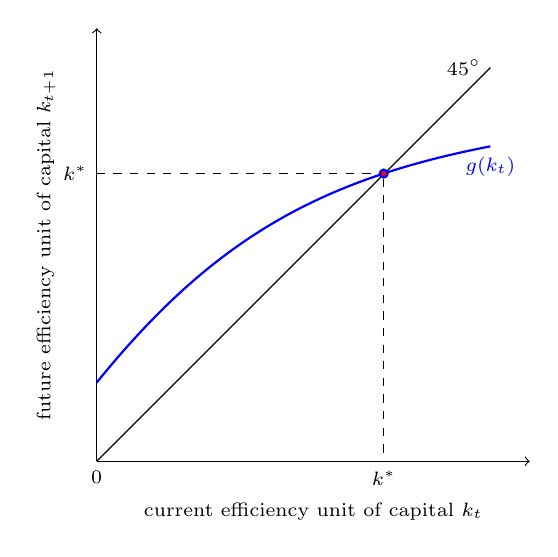
\begin{tikzpicture}[domain=0:5]
                \tikzstyle{every node}=[font=\scriptsize]
                \pgfmathsetmacro{\x}{5};
                \pgfmathsetmacro{\y}{5};
                % \draw[very thin,color=gray, step=0.1] (0,0) grid (\x, \y); % gray grid
                \draw[->] (0,0) node[below]{ $ 0 $  } -- node[below, yshift = -0.4cm]{current efficiency unit of capital $k_{t}$} (\x + 0.5,0) ;   % label x axis
                \draw[->] (0,0) -- node[above, rotate=90, yshift = 0.4cm]{future efficiency unit of capital $k_{t+1}$} (0,\y + 0.5) ;   % label y axis
                \draw[black] plot (\x, \x) node[left]{$45^{\circ}$};
                \draw[thick, blue, yshift = -1cm] (0, 2)
                    to[bend left=20]
                    node[pos=0.21] (b) {}
                    node[pos=0.78,draw,fill=red,circle,inner sep=1pt] (c) {}
                    (5, 5) node[below]{$g(k_{t})$};
                % \draw[shorten >=-1cm, shorten <=-1.5cm, thick, red] (a) -- (b) node[above, yshift=.8cm]{slope $=$ MPC};
                \path (c); \pgfgetlastxy{\xcoord}{\ycoord};
                \coordinate (c_x) at (\xcoord, 0);
                \coordinate (c_y) at (0, \ycoord);
                \draw[dashed] (c_y) node[left]{$k^{*}$}  -- (c) -- (c_x) node[below]{$k^{*}$};
            \end{tikzpicture}
    \task

            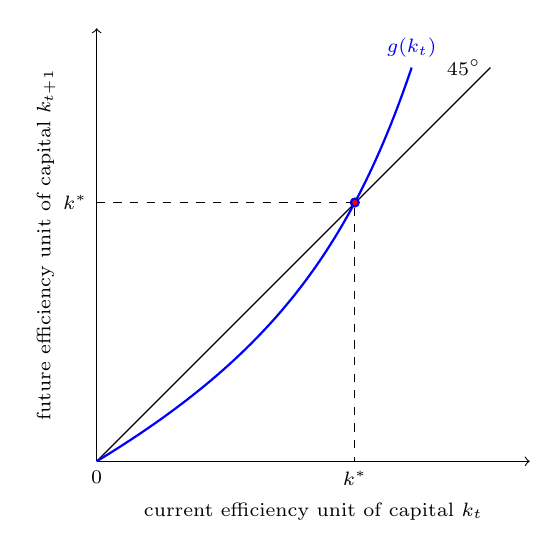
\begin{tikzpicture}[domain=0:5]
                \tikzstyle{every node}=[font=\scriptsize]
                \pgfmathsetmacro{\x}{5};
                \pgfmathsetmacro{\y}{5};
                % \draw[very thin,color=gray, step=0.1] (0,0) grid (\x, \y); % gray grid
                \draw[->] (0,0) node[below]{ $ 0 $  } -- node[below, yshift = -0.4cm]{current efficiency unit of capital $k_{t}$} (\x + 0.5,0) ;   % label x axis
                \draw[->] (0,0) -- node[above, rotate=90, yshift = 0.4cm]{future efficiency unit of capital $k_{t+1}$} (0,\y + 0.5) ;   % label y axis
                \draw[black] plot (\x, \x) node[left]{$45^{\circ}$};
                \draw[thick, blue, yshift = -1cm] (0, 1)
                    to[bend right=20]
                    node[pos=0.21] (b) {}
                    node[pos=0.73,draw,fill=red,circle,inner sep=1pt] (c) {}
                    (4, 6) node[above]{$g(k_{t})$};
                % \draw[shorten >=-1cm, shorten <=-1.5cm, thick, red] (a) -- (b) node[above, yshift=.8cm]{slope $=$ MPC};
                \path (c); \pgfgetlastxy{\xcoord}{\ycoord};
                \coordinate (c_x) at (\xcoord, 0);
                \coordinate (c_y) at (0, \ycoord);
                \draw[dashed] (c_y) node[left]{$k^{*}$}  -- (c) -- (c_x) node[below]{$k^{*}$};
            \end{tikzpicture}
    \task

            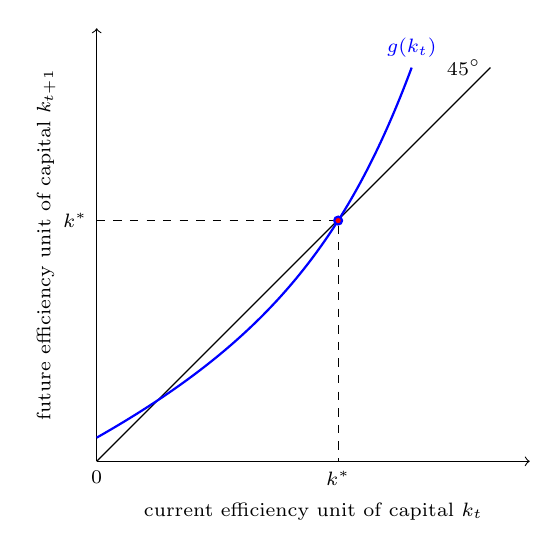
\begin{tikzpicture}[domain=0:5]
                \tikzstyle{every node}=[font=\scriptsize]
                \pgfmathsetmacro{\x}{5};
                \pgfmathsetmacro{\y}{5};
                % \draw[very thin,color=gray, step=0.1] (0,0) grid (\x, \y); % gray grid
                \draw[->] (0,0) node[below]{ $ 0 $  } -- node[below, yshift = -0.4cm]{current efficiency unit of capital $k_{t}$} (\x + 0.5,0) ;   % label x axis
                \draw[->] (0,0) -- node[above, rotate=90, yshift = 0.4cm]{future efficiency unit of capital $k_{t+1}$} (0,\y + 0.5) ;   % label y axis
                \draw[black] plot (\x, \x) node[left]{$45^{\circ}$};
                \draw[thick, blue, yshift = -1cm] (0, 1.3)
                    to[bend right=20]
                    node[pos=0.21] (b) {}
                    node[pos=0.67,draw,fill=red,circle,inner sep=1pt] (c) {}
                    (4, 6) node[above]{$g(k_{t})$};
                % \draw[shorten >=-1cm, shorten <=-1.5cm, thick, red] (a) -- (b) node[above, yshift=.8cm]{slope $=$ MPC};
                \path (c); \pgfgetlastxy{\xcoord}{\ycoord};
                \coordinate (c_x) at (\xcoord, 0);
                \coordinate (c_y) at (0, \ycoord);
                \draw[dashed] (c_y) node[left]{$k^{*}$}  -- (c) -- (c_x) node[below]{$k^{*}$};
            \end{tikzpicture}

    \task

            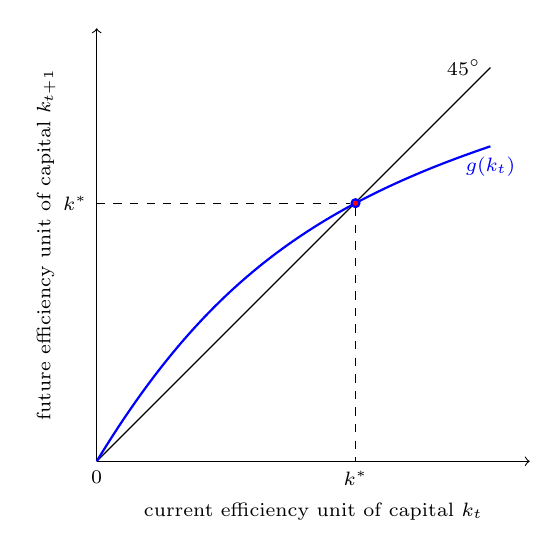
\begin{tikzpicture}[domain=0:5]
                \tikzstyle{every node}=[font=\scriptsize]
                \pgfmathsetmacro{\x}{5};
                \pgfmathsetmacro{\y}{5};
                % \draw[very thin,color=gray, step=0.1] (0,0) grid (\x, \y); % gray grid
                \draw[->] (0,0) node[below]{ $ 0 $  } -- node[below, yshift = -0.4cm]{current efficiency unit of capital $k_{t}$} (\x + 0.5,0) ;   % label x axis
                \draw[->] (0,0) -- node[above, rotate=90, yshift = 0.4cm]{future efficiency unit of capital $k_{t+1}$} (0,\y + 0.5) ;   % label y axis
                \draw[black] plot (\x, \x) node[left]{$45^{\circ}$};
                \draw[thick, blue, yshift = -1cm] (0, 1)
                    to[bend left=20]
                    node[pos=0.21] (b) {}
                    node[pos=0.73,draw,fill=red,circle,inner sep=1pt] (c) {}
                    (5, 5) node[below]{$g(k_{t})$};
                % \draw[shorten >=-1cm, shorten <=-1.5cm, thick, red] (a) -- (b) node[above, yshift=.8cm]{slope $=$ MPC};
                \path (c); \pgfgetlastxy{\xcoord}{\ycoord};
                \coordinate (c_x) at (\xcoord, 0);
                \coordinate (c_y) at (0, \ycoord);
                \draw[dashed] (c_y) node[left]{$k^{*}$}  -- (c) -- (c_x) node[below]{$k^{*}$};
            \end{tikzpicture}
\end{tasks}

\Question What is the $45^{\circ}$ line means in question \ref{kfig}? \answer{B}

\begin{tasks}(3)
    \task $ k_{t+1} > k_{t} $
    \task $ k_{t+1} = k_{t} $
    \task $ k_{t+1} < k_{t} $
\end{tasks}


\Question Among all the figures in the choice of question \ref{kfig}, which graph will the $ g(k_{t}) $ function be \blue{if $ \alpha > 1 $}? \answer{B}

Consider two economies, $a$ and $b$, where economy $b$ has a higher savings rate, \emph{and a higher rate of technological progress}, compared to economy $a$.
In other words, $\gamma_{b}>\gamma_{a}$, and $s_{b}>s_{a}$. Moreover, assume that
\[
\frac{s_{b}}{1+\gamma_{b}}=\frac{s_{a}}{1+\gamma_{a}}\text{,}%
\]
and the rate of population growth is the same ($n_{a}=n_{b}$).

\Question Denote the $ g $ function for both economy as $ g_{a}(k_t) $ and $ g_{b}(k_{t}) $, what is the relationship of two $ g $ function? \answer{B}
\begin{tasks}(1)
    \task $ g_{a}(k_{t}) $ is on top of $ g_{b}(k_t) $, for all $ k_{t} $
    \task $ g_{a}(k_{t}) $ and $ g_{b}(k_t) $ is the same curve
    \task $ g_{a}(k_{t}) $ is below  $ g_{b}(k_t) $, for all $ k_{t} $
    \task $ g_{a}(k_{t}) $ intersects with $g_{b}(k_t) $
\end{tasks}


% Assume both economies have converged to their steady state
% capital by date $T$. If $X_{T}^{a}=X_{T}^{b}$, how
% will income per person differ between economy $a$ and $b$ five years later?
% Explain your answer.

\end{Exercise}


\end{document}

